\documentclass{IEEEtran}
%% PACKAGES %%

\usepackage{amsmath, amsfonts, amssymb, amsthm}
\usepackage{braket}
\usepackage{listings}
\usepackage{geometry}
\usepackage{xcolor}
\usepackage{textcomp}
\usepackage{graphicx}
\usepackage{fancyhdr}
\usepackage{sourcecodepro}
\usepackage{multirow}

%%%%%%%%%%%%%%

\graphicspath{{./images}}

%% LISTINGS CONFIG %%

\definecolor{purple2}{RGB}{153,0,153} % there's actually no standard purple
\definecolor{green2}{RGB}{0,153,0} % a darker green

\lstset{
  basicstyle=\normalsize\ttfamily,   % size of the fonts for the code
  frame = single,
  % Color settings to match IDLE style
  keywordstyle=\color{orange},       % core keywords
  keywordstyle={[2]\color{purple2}}, % built-ins
  stringstyle=\color{green2},%
  showstringspaces=false,
  commentstyle=\color{red},%
  upquote=true,                      % requires textcomp
  breaklines=true,
}

% Title Stuff
\title{ECE296 Lab 8 - Arduino DC Motor Controller}
\author{Chase A. Lotito, \textit{SIUC Undergraduate}}
\date{}

\begin{document}

\maketitle % Makes the title

\section{Introduction} 
% (Brief description of how the lab was setup and the steps you took while completing the tasks given)

This lab experiment was an implementation of a DC motor controller, where we use an H-bridge to control forward and reverse motion, and the Arduino microcontroller to provide input to the H-bridge.

First, we construct a mock DC motor out of two parallel LEDs, in an opposing configuration to show when current flows one direction or the other--this will simulate forward and reverse motion. The use of LEDs instead of an actual motor allows the Arduino to power the entire circuit, without an extra DC power supply. 

Then, the DC motor is connected to the H-bridge, which consists of two PNP transistors and two NPN transistors, the 2N3906 and PN2222A, respectively. When the forward side of the bridge is biased, only current through the forward LED can flow, and vice-versa when the reverse side of the bridge is biased.

Finally, with proper programming of the Arduino, we have four methods: \textit{forward(), reverse(), initialize(),} and \textit{Stop()}. These functions will allow precise control of the DC motor.

\section{Assessment of Design}
% (How did it work in the end? Any problems or missteps along the way? Explain key aspects of design. Attach images of working design.)

Figure \ref{fig:design} shows the final physical implementation of the circuit. 

\begin{figure}[!ht] 
    \centering
    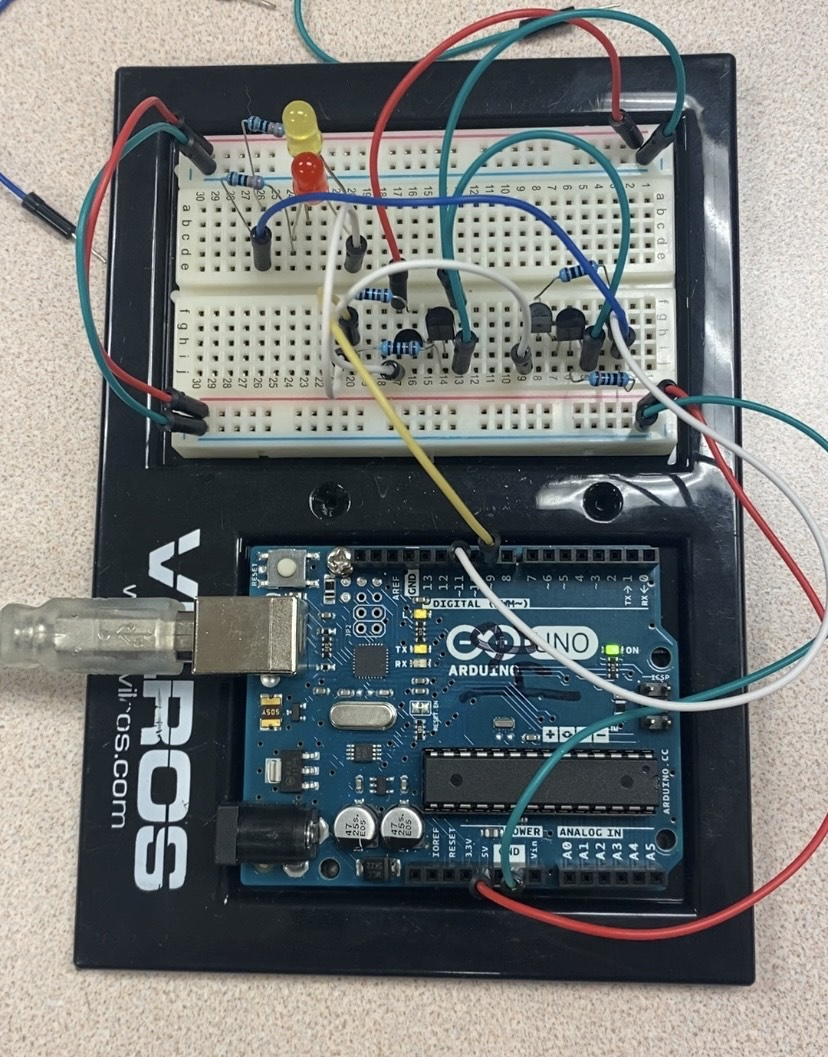
\includegraphics[width = 6cm]{dcmotordesign.jpeg}
    \caption{DC Motor Physical Implementation}
    \label{fig:design}
\end{figure}

Figure \ref{fig:modes} shows the forward and reverse modes in their maximum and minimum intensities. In the code, I have two global variables: \textit{forwardIntensity} and \textit{reverseIntensity}. These variables hold a value between 0 and 255, which allows gradual ramping of the motor. I pass these variables by reference amongst the different functions, and this provides precise control of what state the H-bridge is currently in, and using \textit{delay()} in while loops, I can simulate non-abrupt changes in the motor's motion. Each function utilizes a \textit{while} loop that first checks the current state of either \textit{forwardIntensity} and \textit{reverseIntensity}, and either increments or decrements them according to the specific function. Each time the intensity variables are changed, they are written as a pulse-width-modulated signal via \textit{analogWrite}. 

\begin{figure}[!ht] 
    \centering
    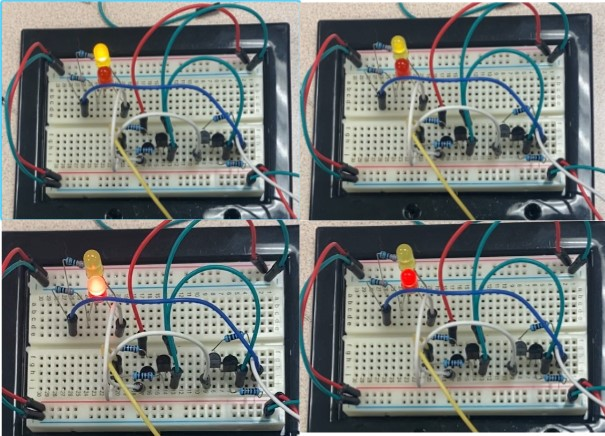
\includegraphics[width = 7cm]{dcmotormodes.jpg}
    \caption{Forward (top) and Reverse (bottom) maximum and minimum intensity.}
    \label{fig:modes}
\end{figure}

\section{Conclusion}
% (What did you learn during this lab? Final thoughts or findings? Did you meet the objectives? Answer any questions given in the lab manual here.)

Overall, this lab shows an extremely practical use of a microcontroller in a control systems application. Motor control is one of the most important aspects of bringing functionality to a mechanical design. Using this configuration, we could even design our own servo motor, which we can make for specific applications standard servos might not fit into.

\section*{Appendix A: Hardware Schematic}

\begin{figure}[!ht] 
    \centering
    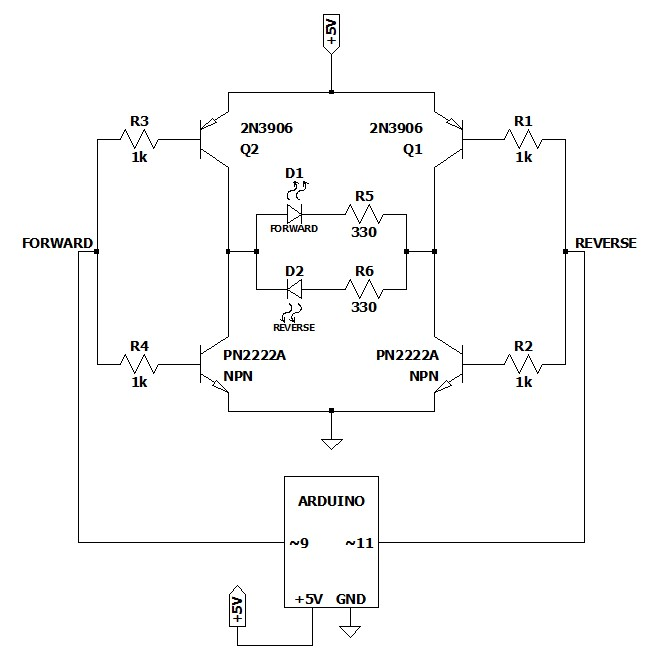
\includegraphics[width = 7.3cm]{dcmotorschematic.jpg}
    \caption{DC Motor Schematic}
    \label{fig:schematic}
\end{figure}

\section*{Appendix B: Code for the Software Developed}

\begin{lstlisting}
// Chase Lotito - Arduino DC Motor Lab

// Pins
const int forwardPin = 9;
const int reversePin = 11;
const int DELAY = 10;

// LED intensity
int forwardIntensity = 0;
int reverseIntensity = 0;

void setup() {
  // put your setup code here, to run once:
  initialize(forwardPin, reversePin);
  Serial.begin(9600);
}

void loop() {
  // put your main code here, to run repeatedly:
  forward(forwardIntensity, reverseIntensity);
  reverse(forwardIntensity, reverseIntensity);
  Stop(forwardIntensity, reverseIntensity);
}

// forward function
void forward(int &fI, int &rI) {
  if (rI > 0) {
    while(rI > 0){
      rI--;
      analogWrite(reversePin, rI);
      delay(DELAY);
    }
  }
  while(fI < 256) {
    fI++;
    analogWrite(forwardPin, fI);
    delay(DELAY);
  }
  return;
}

// reverse function
void reverse(int &fI, int &rI) {
  if (fI > 0) {
    while(fI > 0){
      fI--;
      analogWrite(forwardPin, fI);
      delay(DELAY);
    }
  }
  while(rI < 256){
    rI++;
    analogWrite(reversePin, rI);
    delay(DELAY);
  }
  return;
}

// initialize function
void initialize(int f, int r) {
  // set forward and reverse pins to output
  pinMode(f, OUTPUT);
  pinMode(r, OUTPUT);
  // set pins to ZERO
  digitalWrite(f, LOW);
  digitalWrite(r, LOW);
  return;
}

// stop function
void Stop(int &fI, int &rI) {
  while((fI > 0)) {
    fI--;
    analogWrite(forwardPin, fI);
    Serial.println(fI);
    delay(DELAY);
  }
  while((rI > 0)) {
    rI--;
    analogWrite(reversePin, rI);
    Serial.println(rI);
    delay(DELAY);
  }
  return;
}
\end{lstlisting}

\end{document}
